\documentclass[tikz,border=8pt]{standalone}
\usepackage{amsmath}
\usetikzlibrary{arrows.meta,calc,positioning}
\definecolor{ink}{HTML}{21352F}
\definecolor{teal}{HTML}{087F7B}
\definecolor{gold}{HTML}{C58B2A}
\definecolor{blue}{HTML}{4B77A8}
\definecolor{rose}{HTML}{B65A62}
\begin{document}
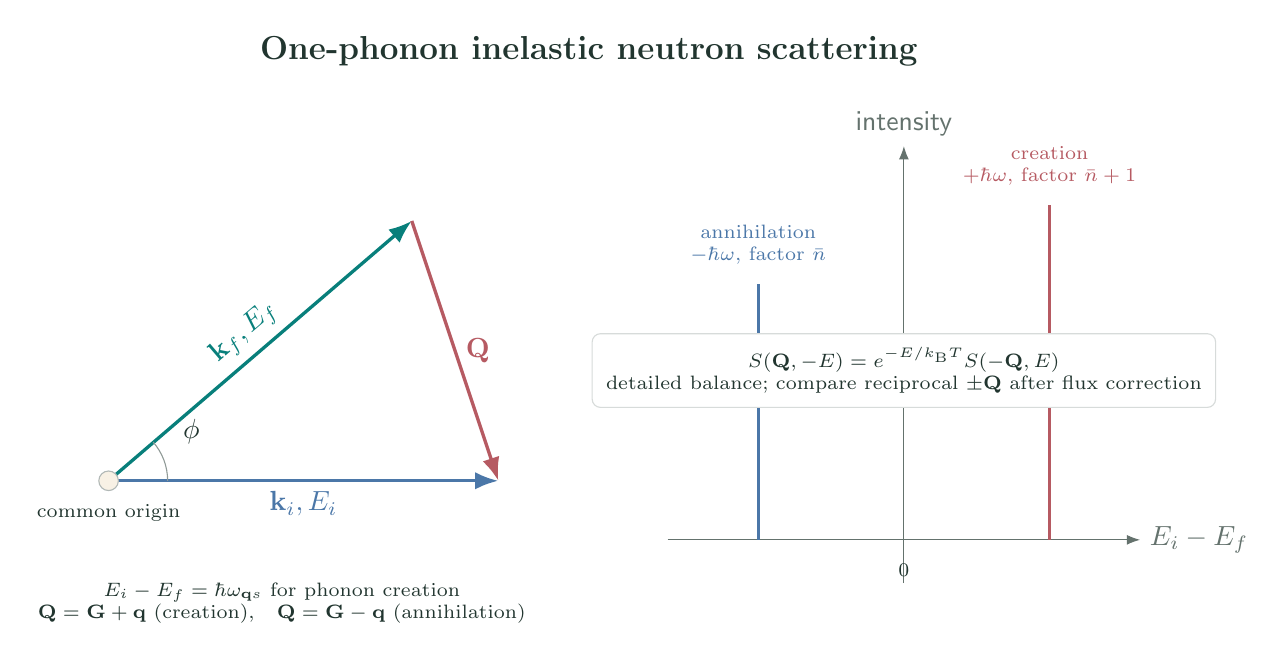
\begin{tikzpicture}[font=\sffamily,text=ink,>=Latex]
  \node[font=\bfseries\large] at (0,4.0) {One-phonon inelastic neutron scattering};
  \coordinate (O) at (-6.1,-1.45);
  \coordinate (Ki) at (-1.15,-1.45);
  \coordinate (Kf) at (-2.25,1.85);
  \draw[->,blue,very thick] (O)--(Ki) node[midway,below] {$\mathbf k_i,E_i$};
  \draw[->,teal,very thick] (O)--(Kf) node[midway,above,sloped] {$\mathbf k_f,E_f$};
  \draw[->,rose,very thick] (Kf)--(Ki) node[midway,right] {$\mathbf Q$};
  \draw[ink!50] ($(O)+(.75,0)$) arc[start angle=0,end angle=41,radius=.75];
  \node at (-5.05,-.82) {$\phi$};
  \node[draw=ink!35,fill=gold!12,circle,inner sep=2.5pt] at (O) {};
  \node[font=\scriptsize,anchor=north] at ($(O)+(0,-.18)$) {common origin};
  \node[font=\scriptsize,align=center] at (-3.9,-3.0)
    {$\displaystyle E_i-E_f=\hbar\omega_{\mathbf q s}$ for phonon creation\\
     $\displaystyle \mathbf Q=\mathbf G+\mathbf q$ (creation),\quad
     $\mathbf Q=\mathbf G-\mathbf q$ (annihilation)};

  \draw[->,ink!70] (1.0,-2.2)--(7.0,-2.2) node[right] {$E_i-E_f$};
  \draw[->,ink!70] (4.0,-2.75)--(4.0,2.8) node[above] {intensity};
  \draw[blue,very thick] (2.15,-2.2)--(2.15,1.05);
  \draw[rose,very thick] (5.85,-2.2)--(5.85,2.05);
  \node[blue,font=\scriptsize,align=center] at (2.15,1.55)
    {annihilation\\$-\hbar\omega$, factor $\bar n$};
  \node[rose,font=\scriptsize,align=center] at (5.85,2.55)
    {creation\\$+\hbar\omega$, factor $\bar n+1$};
  \node[font=\scriptsize] at (4.0,-2.58) {$0$};
  \node[draw=ink!18,rounded corners=3pt,fill=white,inner sep=5pt,align=center,font=\scriptsize] at (4.0,-.05)
    {$\displaystyle S(\mathbf Q,-E)=e^{-E/k_{\rm B}T}S(-\mathbf Q,E)$\\
     detailed balance; compare reciprocal $\pm\mathbf Q$ after flux correction};
\end{tikzpicture}
\end{document}
